% Train-time ablation section + figure. Numbers from docs/01 §ABL-Q8; figure by paper/plot_ablation.py.
% Runs: iclr_rlh_ablq8_yyn (think on) / iclr_rlh_ablq8_ynn (think off), target = the no-reflection Qwen3-8B checkpoint.

\subsection{Train-Time Ablation of Self-Reflection}
\label{sec:train_time_ablation}

The ablation in Section~\ref{sec:think_ablation} disables reasoning at inference on a model that was trained to reason,
so the degradation it measures may reflect a train/inference mismatch rather than the value of the reflection itself.
We therefore run the ablation on the \emph{training} side: we rebuild the SRFT dataset with every reflection removed,
keeping the injected contexts, the expert trajectories and the supervised optimal actions untouched, and fine-tune
Qwen3-8B with the recipe used for SR-Agent, changing only the data. The resulting model is exposed to exactly the same
adversarial experience as SR-Agent and is trained to take the same actions; it is simply never told why those actions
are preferable. Comparing the two therefore isolates the contribution of the self-reflection supervision.

We evaluate the ablated model under the RL-Hammer adaptive attack in two inference settings, with the thinking mode
held consistent between attacker training and target evaluation: with thinking enabled, matching how the base model and
SR-Agent are evaluated, and with thinking disabled, matching how the ablated model was trained. Reporting both removes
the confound that motivated this experiment: if the two settings agree, the outcome cannot be attributed to the model
being evaluated outside its training distribution.

\begin{figure}[t]
  \centering
  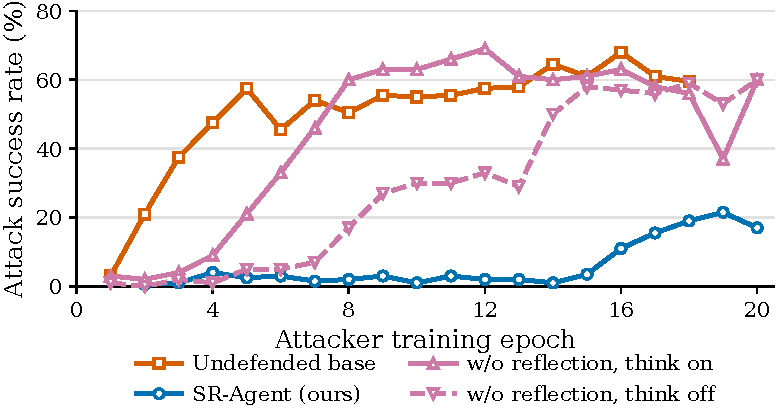
\includegraphics[width=0.72\linewidth]{fig_ablation.pdf}
  \caption{\textbf{Train-time ablation of self-reflection under adaptive attack (Qwen3-8B).} Attack success rate over
  attacker training epochs. The undefended base and SR-Agent are each the mean of two independent attacker runs; the two
  ablation curves are single runs of the same checkpoint and differ only in the target's thinking mode, which is held
  consistent between attacker training and evaluation. Lower is better.}
  \label{fig:train_time_ablation}
\end{figure}

Figure~\ref{fig:train_time_ablation} shows the result. Removing the reflection supervision returns the model to the
robustness of no defence at all: the ablated model ends at $60\%$ ASR with thinking enabled and $60\%$ with thinking
disabled, against $59.5\%$ for the undefended Qwen3-8B, while SR-Agent trained on the same trajectories ends at
$17.0\%$. The agreement between the two inference settings is what makes the comparison interpretable --- the ablated
model is equally vulnerable whether or not it is asked to think at inference, so its collapse follows from the missing
reflection supervision and not from a distribution shift at evaluation time.

This isolates where the robustness comes from. Exposure to compromised trajectories, together with supervision on the
correct non-hijacked action, is by itself not enough: a model trained on exactly that signal is broken by the adaptive
attacker as readily as an undefended one. What survives the attacker's optimisation is the reflective supervision ---
learning to identify the injected instruction and to reason about why the optimal action is preferable to the hijacked
alternatives. Consistent with this reading, the ablated model's attacker reward rises sharply midway through training,
the signature of an attacker that has found a working strategy, whereas the same attacker training against SR-Agent
stays near the floor for most of its schedule.
